% SPDX-License-Identifier: CC-BY-SA-4.0
% Author: Matthieu Perrin
% Part: <Nom de la partie>
% Section: <Nom de la section>
% Sub-section: <Nom de la sous-section>  % (facultatif, laisser vide si non utilisé)
% Frame: <Titre de la slide>

\begingroup

\begin{frame}{Un exemple : le \og Subset-Sum Problem\fg}

  \Probleme{Subset-Sum}{
    Un ensemble fini d'entiers $E \subset \mathbb{Z}$
  }{
    Existe-t-il $S \subseteq E$ non vide tel que $\displaystyle\alert{\sum_{n\in S} n = 0}$ ?
  }

  \begin{exampleblock}{Exemple}
    \centering
    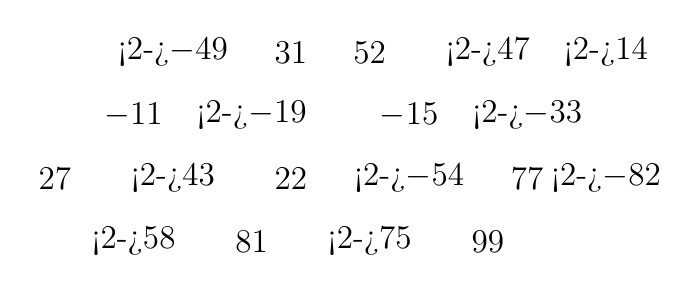
\begin{tikzpicture}[y=8mm]\large
      \node at (5,3)   {$31$};
      \node at (2,1)   {$27$};
      \node at (3,2)   {$-11$};
      \node at (4.5,0) {$81$};
      \node at (5,1)   {$22$};
      \node at (6.5,2) {$-15$};
      \node at (7.5,0) {$99$};
      \node at (8,1)   {$77$};
      \node at (6,3)   {$52$};
      \node at (7.5,3) {\alert<2->{$47$}};
      \node at (9,1)   {\alert<2->{$-82$}};
      \node at (3,0)   {\alert<2->{$58$}};
      \node at (3.5,1) {\alert<2->{$43$}};
      \node at (4.5,2) {\alert<2->{$-19$}};
      \node at (6,0)   {\alert<2->{$75$}};
      \node at (6.5,1) {\alert<2->{$-54$}};
      \node at (8,2)   {\alert<2->{$-33$}};
      \node at (9,3)   {\alert<2->{$14$}};
      \node at (3.5,3) {\alert<2->{$-49$}};
    \end{tikzpicture}
  \end{exampleblock}
  
  \pause
  \begin{alertblock}{Réponse}
    \begin{itemize}
    \item $47-82+58+43-19+75-54-33 + 14 -49 = 0$
    \end{itemize}
  \end{alertblock}

\end{frame}

\endgroup
